\epigraph{
To mention all the mineral substances in which I have found these molecules, would be tedious; and I shall confine myself in this summary to an enumeration of a few of the most remarkable. These were both of aqueous and igneous origin, as travertine, stalactites, lava, obsidian, pumice, volcanic ashes, and meteorites from various localities. Of metals I may mention manganese, nickel, plumhago, bismuth, antimony, and arsenic. In a word, in every mineral which I could reduce to a powder, sufficiently fine to be temporarily suspended in water, I found these molecules more or less copiously; and in some cases, more particularly in siliceous crystals, the whole body submitted to examination appeared to be composed of them.}{\textbf{Robert Brown, on what we now call Brownian particles}}

\section{Brownian motion}
Brownian motion is the motion that occurs when looking at microscopic particles that are suspended in a fluid, this motion is highly random and is due to molecules in the fluid colliding with the particle trillions of times per second. Brownian motion occurs on the micro-meter to nano-meter scale \cite{KellerBustamante2000,Reimann2001}, particles of this size are constantly bombarded by the environment causing some people to use the term molecular hurricane \cite{Astumian2007}, amazingly though, some systems in biology and in the laboratory are able to create directed motion and draw energy from this chaotic environment \cite{Reimann2001}. In principle if one knew the momenta and positions of all particles in a system, then one could use Newtonian mechanics to fully predict the future state of the system. However, for systems of interest in this project, we will be looking at systems with particle number on the order of Avagadro's number ($N \sim 10^{23}$). With systems of this size, a Newtonian description is completely impractical, so instead we will use a statistical approach, in this view the motion of a single Brownian particle suspended in a fluid at a given temperature (which we will call the bath) is random, we explain this random motion in Figure \ref{fig:brownianMotion}.

\begin{figure}
	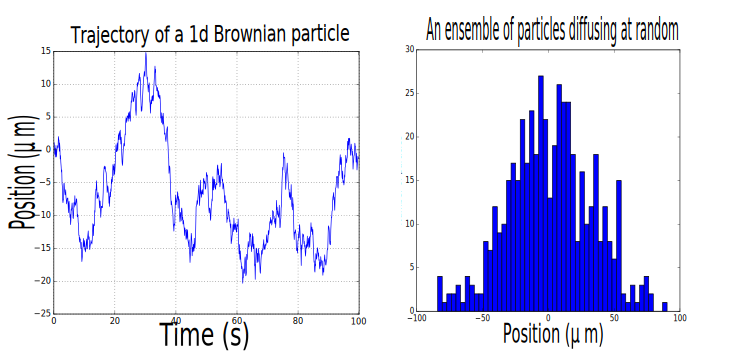
\includegraphics[width=0.8\textwidth]{brownianMotion}
	\caption{\textbf{Cartoon demonstration of Brownian motion.} (a) Trajectory of a single tagged Brownian particle, the particle is being forced around randomly by the molecular hurricane, since there is no nett force on the particle, we find that the particle makes no nett progress over time. (b) An ensemble of Brownian particles simulated for 100 seconds, here we see that the mean movement is zero because there is no background force on the particles, this statistical nature of the particles motivates us to view the particles in a probabilistic sense. (c) The particles can be placed in a potential (for example charged particles in an electric field), initially the particles were all located at $x = 0$, after some time we find that the particles have moved to a lower potential energy state and that they tend to situate at the bottom of the wells in the potential. These locations can be approximated by parabolas, it can be shown that in this case, the particles will decay into a Gaussian distribution \cite{UhlenbeckOrnstein1930} as we can see in the figure. (d) Zoomed in cartoon of a particle about to jump over a barrier, in Newtonian mechanics the particle would need enough potential energy to simply roll over the barrier, however in this project we will be in the over-damped regime where the particles have no inertia, in order for the particle to get over the barrier there will need to be an event that occurs where many particles will hit the particle on its right hand side. This will cause the bath to lose some energy as heat as shown in the figure and this heat will be the source of the thermal interactions that we will talk about in ~\autoref{Smoluchowski}  \label{fig:brownianMotion}}
\end{figure}


Brownian motion was first observed by Robert Brown in 1827 \cite{Brown1828}, in these observations, Brown saw that microscopic particles (for example pollen grains) were in constant motion. He noticed that this motion was still present in inorganic material including granite and ground up Sphinx bones.
Over half a century later, Einstein showed that Brownian motion was due to constant bombardment by water molecules in the surrounding environment \cite{Einstein1905}, Einstein's theory of Brownian motion was then experimentally verified by Perrin \cite{Perrin2013}.

\begin{figure}[tb]
	\begin{subfigure}{0.49\textwidth}
		\includegraphics[width=\columnwidth]{tiltedPeriodicBoringInit}
		\caption{\label{fig:Init}}
	\end{subfigure}
\begin{subfigure}{0.49\textwidth}
		\includegraphics[width=\columnwidth]{tiltedPeriodicBoringFinal}
		\caption{\label{fig:Final}}
\end{subfigure}
\caption{Schematic showing the probability density of particles diffusing in a one dimensional tilted periodic potential at a fixed temperature. We see that the particles tend to drift down the potential as they diffuse, this drift will be called the current $J$ which we will quantify in section ~\autoref{Smoluchowski}. In section \ref{dimensionless}, we will define the dimensionless time scale and length scale used in the calculations for this figure.}
\label{fig:Schematic}
\end{figure}

Brownian particles can be described stochastically by the Langevin equation which is essentially Newton's second law with a random force applied to it, we can write this as:
\begin{equation}
-m \ddot{x}(t) = \gamma \dot{x} (t) + F(t) + \xi(t) 
\end{equation}
Where $\gamma$ is the viscous friction coefficient of the Brownian particle, is an external force on the particle and $\xi(t)$ is Gaussian white noise with zero mean and has auto-correlation given by $\langle \xi(t) \xi(s) \rangle = 2 \gamma k_B T \delta(t - s)$. $\xi(t)$ is the thermal noise of the environment, this is the force produced by the collisions of the Brownian particle with particles in the environment.
The regime of Brownian motion that we will discuss is the so called over-damped limit, in this the mass of the particle is so small that we ignore the inertia of the particle. Therefore, all of the energy of the system is quantified by the potential energy of the particle and the thermal energy of the bath \cite{Streater1997,Streater1997a,Streater2000,Streater1997b}. The over-damped regime of a Brownian particle can be described stochastically by the Langevin equation 
\begin{equation}
	\gamma \dot x(t) = F(x(t)) + \xi(t)  \label{eqn:langevin}
\end{equation}
This is essentially the stochastic view of Brownian motion, as mentioned earlier we can also describe Brownian motion by following the evolution of the probability distribution of a single Brownian particle.

The probabilistic view of Brownian motion is shown in Figure \ref{fig:Schematic}, here we see the same physical situation as depicted in part (c) of Figure \ref{fig:brownianMotion}. The key difference is that in Figure \ref{fig:Schematic} we do not have any knowledge of the individual particles in the ensemble, but instead we only know about the probability distribution that describes them. The situation in Figure \ref{fig:Schematic} is described by the Smoluchowski equation \cite{Gardiner2009}, from now on we will use the Smoluchowski equation to model a Brownian particle, however it is useful to keep in mind that the underlying dynamics are stochastic. The Smoluchowski equation can be written as:

\begin{equation}
\frac{\partial P(x, \, t)}{\partial t} =  \gamma^{-1} \frac{\partial}{\partial x} \left (P(x, \, t) \frac{\partial V(x, \, t)}{\partial x} + k_B T(x,  \, t) \frac{\partial P(x, \, t)}{\partial x} \right )
\end{equation}
Where $P(x, \, t)$ is the probability that the particle is at $x$ at time $t$, $V(x, \, t )$ is the potential, $T(x, \, t)$ is the temperature of the environment, $\gamma$ is the viscous drag coefficient of the particle and $k_B$ is the Boltzmann constant. From now on we will be dealing with potentials that do not change with time, so we will write $V(x, \, t)$ as $V(x)$. The Smoluchowski equation describes precisely the same physical situation as equation \ref{eqn:langevin}. Intuitively, the first term of the equation represents the force that the potential applies on the particle and the second term represents the diffusion of the particle due to thermal noise.

\section{Brownian motors}
Brownian motors are devices that can use stored chemical energy to create directed motion on a microscopic scale and are ubiquitous in biology where, by transforming energy from one degree of freedom to another, they are used to perform important tasks in cells \cite{PhillipsQuakeMay2006, Magnasco1994,Nelson2014}. Recently, thanks to improvements in imaging techniques, researchers have been able to make highly detailed images of these motors and their working components \cite{YiWeiChang2016}. As well as being able to crank a rotor in the in the fashion of a traditional motor, Brownian motors are also able to pump ions against a gradient and translocate molecules \cite{Magnasco1994, Reimann2001, Leibler1993, leibler1990physical}. Artificial Brownian motors have been investigated in the laboratory, for example Ref \cite{BlickleBechinger2011} created a stochastic heat engine by placing a single colloidal particle in a time dependent optical trap. Likewise, Ref \cite{Pedro2014} placed a colloidal particle in an optical tweezer and drove the particle with explosive vaporization of the surrounding liquid, thus demonstrating a thermal mechanism for Brownian motors. Ref \cite{JoelBader1999} placed DNA molecules in a time dependent potential to transport the molecules. Brownian ratchets capable of walking along a track have been implemented in the laboratory recently  ~\cite{Wang2010,DeliusGeertsemaLeigh2010,DeliusGeertsemaLeighEtAl2010}. In order to improve on these designs and to approach the efficiency present in nature, we will have to understand the physics of Brownian dynamics very clearly.

The name Brownian motors is not a misnomer, a Brownian motor can be modeled as a Brownian particle diffusing over a potential \cite{Reimann2001}, in the case of Brownian motion it is natural to think of the particle moving in a spatial coordinate $x$, however in the case of Brownian motors the interpretation of the coordinate $x$ is more abstract. In general $x$ will be a degree of freedom for the system, examples include reaction coordinates for a chemical reactions, or in the case of a rotary motors, the angle of the motor itself.

\section{Classes of Brownian motors} \label{BrownianMotorClasses}
Here we will discuss different classes of Brownian motors and their relationship to the project. Different types of Brownian motors have been explored in the literature, including the Feynman ratchet \cite{Feynman1963}, the Landauer blowtorch \cite{Landauer1988}, thermal ratchets \cite{Pedro2014}, time dependent potentials \cite{JoelBader1999,BlickleBechinger2011} and on tilted periodic potentials \cite{Leibler1993,Magnasco1994}.

\subsection{Feynman ratchet and pawl}
\begin{figure}
	\center
	\includegraphics[width=0.6\columnwidth]{g_ratchet}
	\caption{\textbf{The Feynmann ratchet and pawl \cite{Feynman1963}.} The ratchet is located in a bath at temperature $T_1$ and the vanes are in a bath at temperature $T_2$.  (Figure taken from http://pof.tnw.utwente.nl/research/granular/ratchet) \label{fig:feynmannRatchet}}
\end{figure}
The Feynman ratchet was initially discussed in the Feynman lectures \cite{Feynman1963}, it is an intuitive picture of how a motor may work at the microscopic scale and was at first thought to be able to achieve Carnot efficiency, however closer analysis showed that this was not possible \cite{ParrondoEspanol1996}. The system works as follows, we have two boxes that are thermally insulated from one another that are connected by an axle that can rotate, these two boxes are at temperature $T_1$ and $T_2$ where in general $T_1 \neq T_2$. In one box there is a ratchet and pawl connected to the axle that makes it easy for the axle to turn one way (say clockwise), but hard to turn the other way (anti-clockwise). In the other box the axle is connected to vanes that are being buffeted by a gas. The motion of the vanes are random since they are dictated by Brownian motion, so the purpose of the ratchet and pawl is to rectify the Brownian motion of these vanes. One may think that this could be used to extract energy from the environment (for example by using the axle to lift a weight), this is true but one may not attain Carnot efficiency. The problem is that the ratchet and pawl themselves will also be subject to random motion so sometimes the pawl will be lifted allowing the axle to turn anti-clockwise.

In the case where $T_1 = T_2$, the pawl will be lifted just as frequently as the vanes are turned and the system will make no net progress, this occurs despite the asymmetry of the ratchet. In the case where $T_2 > T_1$, the vanes will be moving quite frequently and we will find that work can be extracted from the system. On the other hand, when $T_2 < T_1$ the vanes will be turning infrequently but the pawl will spend most of its time in the up position, allowing the axle to turn either direction, thus causing the ratchet to have no net motion. Feynmann then reasoned that when $T_2 > T_1$, the system could achieve Carnot efficiency in the quasi-static limit where the net motion goes to zero, this is in close analogy to a macroscopic heat engine, however the reasoning turned out to be flawed. The flaw in Feynmann's reasoning  was that he did not consider the intrinsic irreversibility of the system, one must note that although the two boxes may be thermally insulated, they will still exchange heat through the axle itself. In order for Carnot's efficiency to be realized, the process must be reversible, so Feynmann's ratchet cannot attain Carnot efficiency.  

To model the Feynman ratchet and measure it's efficiency, we will need two degrees of freedom \cite{M.W.Jack2016}, this is beyond the scope of this project because we will only simulate systems with one degree of freedom.

\subsection{Landauer's blowtorch} \label{landauersBlowtorch}
\begin{figure}[tb]
%	\center
%	\textbf{Landauer's blowtorch}
%	\vspace{0.5cm}
	\begin{subfigure}{0.42\textwidth}
		\includegraphics[width=\columnwidth]{landauersBlowtorchA}
		\caption{\label{fig:landauerA}}
	\end{subfigure}
	\begin{subfigure}{0.42\textwidth}
		\includegraphics[width=\columnwidth]{landauersBlowtorchB}
		\caption{\label{fig:landauerB}}
	\end{subfigure}
	\begin{subfigure}{0.12\textwidth}
		\includegraphics[width=\columnwidth]{landauersBlowtorchLegend}
	\end{subfigure}

\caption{\textbf{Landauer's blowtorch in a bi-stable potential}. (a) we see that if the particles are left for a long enough time, then they will reach an equilibrium where the population in the upper well is less than that in the lower well. In (b) we see that if the temperature in the upper well is lower than that of the lower well, then the euilibrium concentrations are drastically altered.}
\label{fig:landauersBlowtorch}
\end{figure}
The Landauer blowtorch scheme involves a temperature that varies in space \cite{Landauer1988}. The principle is shown schematically in Figure \ref{fig:landauersBlowtorch}, in this figure the temperature is held fixed by an external heat source and can be made to vary along the potential. The steady state probability distribution was calculated using techniques that are described in ~\autoref{SteadyState}, in reference to this phenomena Landauer says that \cite{Landauer1988}  ``The relative occupation of competing states of local stability is not determined solely by the characteristics of the locally favored states, but depends on the noise along the whole path connecting the competing states.'' The reason that particles move against the potential gradient is that where the potential is heated, the particles become more agitated, therefore we should expect that the probability of finding a particle in a hot region is small. A common analogy due to G. E. Hinton is pebbles on a driveway, if one places pebbles on a driveway in a uniform fashion, then after some time one will find that the pebbles will pile up on the side of the driveway where there is no traffic. This occurs despite the fact that the car exerts no net sideways force on the pebbles, the explanation of this phenomena is that the car is agitating the pebbles in the center effectively at random, but once the pebbles leave the center they experience no agitation (zero temperature), so they will stay in place. This has caused some authors to describe the temperature as an effective potential \cite{Gardiner2009, Kampen1988}, in particular \cite{DasDasBarikEtAl2015} report a so called reverse Landauer blowtorch effect. In their paper, the authors report that if one begins with particles in the upper well of a bi-stable potential, then as the particles move to the lower well, they will reduce the temperature of the upper well. In section ~\autoref{Kramers}, we will discuss the reverse Landauer blowtorch in more detail. The Landauer blowtorch is an important system because it clearly demonstrates that temperature gradients in stochastic systems need to be accounted for.

\subsection{Tilted periodic potentials}
The tilted periodic potential (Figure \ref{fig:Schematic}) is of particular interest for this project because it can be used to model biological motors \cite{Leibler1993,Magnasco1994}. In this model, the potential can be a very complicated function of space despite the fact that temperature is held fixed. One way to model Brownian motors of this class is to think of a reaction coordinate $x$ that describes the conformation of a molecule in a chemical reaction. An example of this is the reaction ATP $\rightleftharpoons$ ADP + P, where ATP is adenosine tri-phosphate, ADP is adenosine di-phosphate and P is a lone phosphate molecule. This reaction coordinate is then coupled to a mechanical coordinate $y$ so that each time that a reaction takes place, the motor will move in some way. Since this is a chemical reaction, the free energy will be decreased as time moves forwards. So a system that has a potential that is periodic in $x$ is not sufficient to describe this situation, we will need to ``tilt" the potential by adding a forcing $f$. The value of $f$ will depend on the $\Delta G$ of the reaction (i.e. how far out of equilibrium the reaction is). It is shown in \cite{Magnasco1994} that this can be modeled by the two dimensional Smoluchowski equation. In this project we will only be modeling the one dimensional Smoluchowski equation, so we will have to consider the case where $x$ and $y$ are tightly coupled. An example of tight coupling is the kinesin motor \cite{Leibler1993} that is used in cells to transport molecules. The kinesin motor is strongly bound to a track that it ``walks" along, on each step the motor will hydrolyze an ATP molecule using the reaction shown above. This reaction liberates about $12 k_B T$ Joules of energy that the motor uses to move forward. Kinesin motors are able to take many steps forward while taking few steps backwards all while falling off their track very infrequently \cite{BlockSM1990}.
\section{Aims}
The aims of this project are as follows:
\begin{itemize}
\item{Determine a consistent physical description of Brownian motion involving self-induced temperature gradients, this description must be consistent with the laws of thermodynamics and should be consistent with previous models in limiting cases}
\item{Develop analytical and numerical methods for solving the system}
\item{Explore the behavior of this system and determine the effect of self-induced temperature gradients on Brownian dynamics}
\end{itemize}
\section{Student contributions}
The work of this honors project is as follows:
the code for the project can be found at \href{url}{https://github.com/JackDevine/Honours2016}, as well as the code we have included a script for testing the numerics to make sure that they are working as well as some Jupyter notebooks to help explain how the code works and how to use it.
